\section{Firmware}
\label{Firmware}
The Attiny861 is running a Firmware, based on a basic Moore state machine\footurl{https://en.wikipedia.org/wiki/Moore_machine} with eight states. Each state performs an essential function, with distinct sound and status LED outputs. More about the state machine in \cref{State Machine}. The code was written in \textit{C++}(Arduino \textit{C++}) inside the Arduino IDE. Please note that the firing sequence, that controls the pyrotechnic show, is refereed to as program.

\subsection{Pinout}

\begin{figure}[!ht]
    \centering
    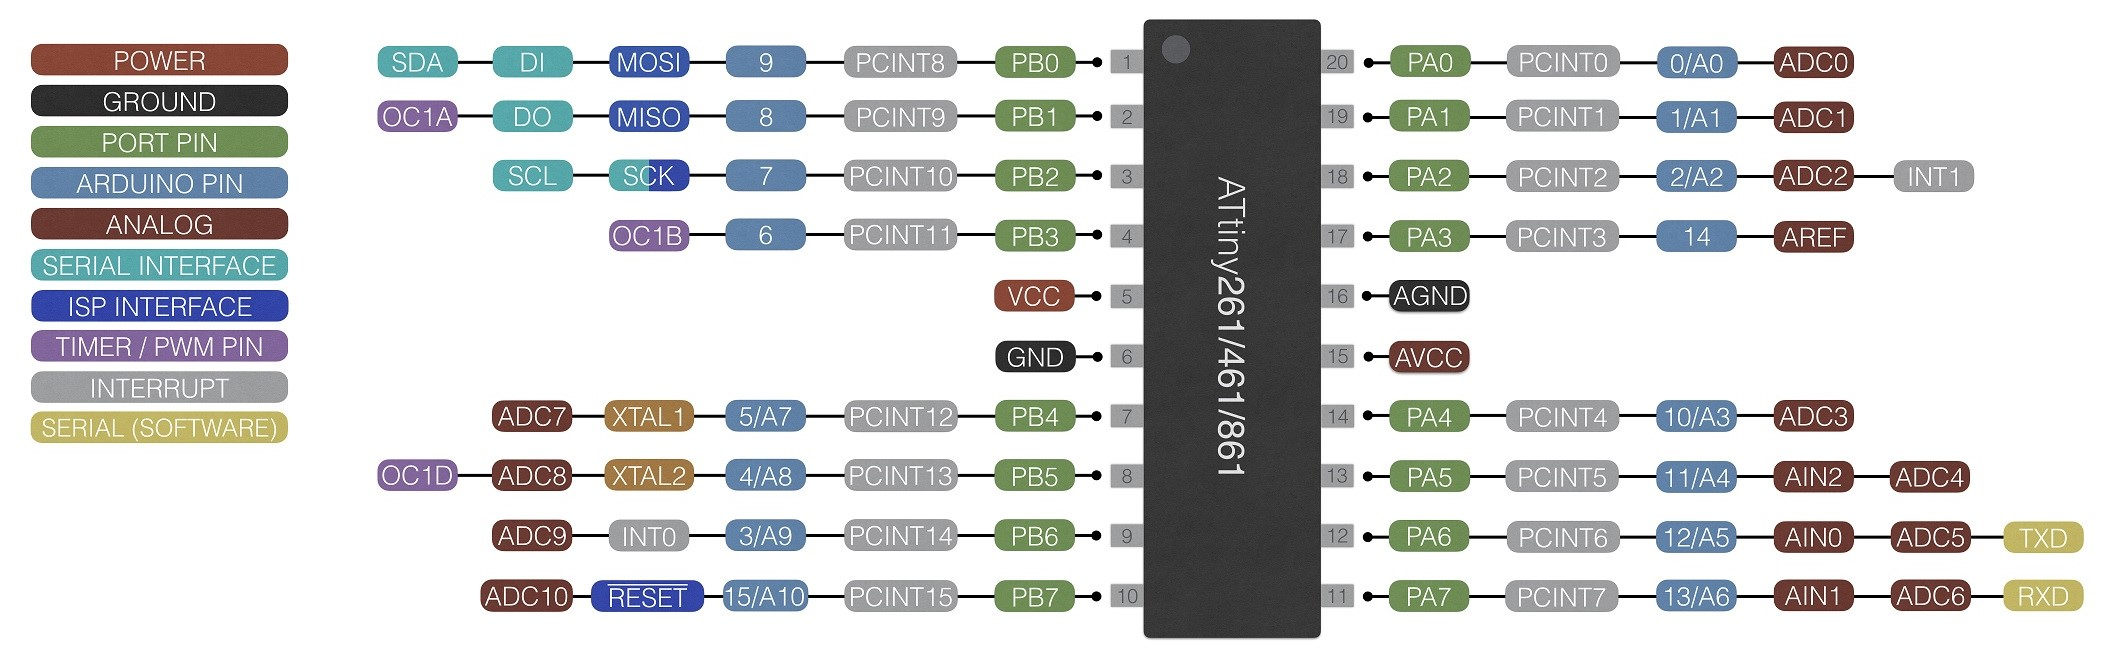
\includegraphics[width=13cm]{./Figures/attiny861_pinout.jpg}
    \caption{Pinout of the Attiny861 µC.}
    \label{fig:attiny861_pinout}     
\end{figure}

\sourceurl{}{fig:attiny861_pinout}{https://github.com/SpenceKonde/ATTinyCore}

\noindent All pins, shown in \Cref{fig:attiny861_pinout}, of the µC were used except pin 18 as this is the reset pin. The pin descriptors, used inside the firmware, are listed in \cref{tab:pinio}.

\begin{table}[!ht]
    \centering
	\begin{tabular}{|l|l|l|l|}\hline
Pin & Name               & Type &Description \\ \hline \hline
3   & MODUL\_DATA        & OUT & Dataline for serial data transmission\\ \hline
4   & MODUL\_CLK         & OUT & Clock signal for serial data transmission\\ \hline
2   & TRIGGER\_FIRE      & INT & Receives the trigger signal from the trigger\\ \hline
0   & TRIGGER\_ARMED     & IN & High if trigger is armed\\ \hline
1   & TRIGGER\_CONNECTED & IN & High if trigger is connected           \\ \hline
8   & TRIGADD\_A0        & OUT & Address line for selecting the ignition module\\ \hline
9   & TRIGADD\_A1        & OUT & Address line for selecting the ignition modul\\ \hline
10  & TRIGADD\_1E        & OUT & Enable line for selecting the ignition modul\\ \hline
11  & TRIGADD\_2E        & OUT & Enable line for selecting the ignition modul\\ \hline
12  & STATUS\_RED        & OUT & Turns on the red status LED on the controller\\ \hline
13  & STATUS\_GREEN      & OUT & Turns on the green status LED on the controller\\ \hline
12  & STATUS\_PIEP       & OUT & Turns on the buzzer on controller and trigger\\ \hline
14  & THIS\_ARMED        & IN & High if controller is armed\\ \hline
7   & RX                 & IN & Receive signal for serial TTL communication\\ \hline
6   & TX                 & OUT & Transmit signal for serial TTL communication\\ \hline
	\end{tabular}
	\caption{Signal descriptions of all pins used of the Attiny861}
	\label{tab:pinio}
\end{table}

\pagebreak

\subsection{Setup}
\label{FSetup}

\noindent The pinout listed in \cref{tab:pinio} gets configured inside the \textit{setup} function(See \cref{lst:iosetting}) which executes once on boot. Inside the same function call, the interrupt will be configured, to invoke a function called \textit{fire}, if the pin voltage level changes from low to high on pin 2.  Furthermore, the baud rate for the TTL serial communication is set to \textit{57600}. More about the serial communication in \cref{Program Mode}.\\

\lstinputlisting[frame=l,captionpos=b,firstline=112,lastline=128,caption=Code configuring the IO pins of the Attiny861. ,label=lst:iosetting]{../../Firmware/ZK_48_Firmware/ZK_48_Firmware.ino}

\noindent All the register of the ignition modules are cleared during \textit{setup}, by calling the \textit{transmitData}(See \cref{Serial Data Transmission}) function with an out of range index(See \cref{lst:cleardisable}). This sets all ignition modules internal shift registers to 0. This is done due safety reasons, to prevent accidental premature firing, as already stated in \cref{Components of the Controller} "Arm safety circuit". For the same reason, the \textit{setModule} function(See \cref{Ignition Module addressing}) is used to disable all ignition modules. The program endpoint is also read from the internal EEPROM(More about that in \Cref{Program Mode}).\\

\lstinputlisting[frame=l,captionpos=b,firstline=130,lastline=132,caption=Code clearing and disabling ignition modules and reading the program endpoint. ,label=lst:cleardisable]{../../Firmware/ZK_48_Firmware/ZK_48_Firmware.ino}

\noindent The code snipped shown in \Cref{lst:clockdiv} is also executed in the setup function. Without this code in \cref{lst:clockdiv} the firmware would only execute at a eighth of normal speed. This means, a delay of $10ms$ takes $80ms$. This increase of the delay was measured, by programming the Attiny861 to output a $10ms$ pulse which got measured by a oscilloscope. The oscilloscope measured $80ms$ instead of $10ms$. Research led to a forum post where the code in \cref{lst:clockdiv} was found and subsequently tested, which proved to be successful in restoring the correct timing. Why this increase in delay occurs in the first place is unknown.

\lstinputlisting[frame=l,captionpos=b,firstline=106,lastline=109,caption=Code for removing the clock division factor.,label=lst:clockdiv]{../../Firmware/ZK_48_Firmware/ZK_48_Firmware.ino}

\sourceurl{ the Code in}{lst:clockdiv}{https://community.platformio.org/t/attiny-8mhz-wrong-timing\\-in-delay-fastled-and-neopixel/24992/3}

\pagebreak

\subsection{Ignition of a Port}

\lstinputlisting[frame=l,captionpos=b,firstline=290,lastline=299,caption=Ignition function for setting of a bridge wire detonator given a port index and ignition module,label=lst:ignitionfunc]{../../Firmware/ZK_48_Firmware/ZK_48_Firmware.ino}

\noindent The function \textit{ignite}, shown in \cref{lst:ignitionfunc}, will set of a bridge wire detonator by the principle explained in \cref{Ignition Module work} "Controlling the Ignition Circuits". On line 3 in \cref{lst:ignitionfunc} the port gets set on all ignition modules and on line 4 the correct ignition modules gets selected, thereby firing the port. After a delay called the ignition time, which is the time current runs through the detonator, all modules get unselected and the ignition modules registers are cleared.\\

\subsubsection{Ignition Module addressing}
\label{Ignition Module addressing}

\lstinputlisting[frame=l,captionpos=b,firstline=29,lastline=47,caption=Bit array for controlling the DMUX,label=lst:dmux_map]{../../Firmware/ZK_48_Firmware/ZK_48_Firmware.ino}

\noindent A two dimensional byte array, behaving like lookup table, is used for controlling the two DMUX onboard the controller, which addresses the ignition modules. Every row of the constant \textit{module\_resolve} contains a unique bit pattern for each module. The values are the result of the wiring of the DMUX shown in \cref{Ctrlcircuit}. This lookup table like design allows the ignition modules to be addressed by just a single integer value. Line 2 till 5 in \cref{lst:dmux_map} define aliases for mapping the column in \textit{module\_resolve} (as shown in line 10) onto the correct outputs \textit{TRIGADD\_A0}, \textit{TRIGADD\_A1}, \textit{TRIGADD\_E1}  and \textit{TRIGADD\_E2}. 

\lstinputlisting[frame=l,captionpos=b,firstline=281,lastline=287,caption=Code selecting a module by its index,label=lst:dmux_controll]{../../Firmware/ZK_48_Firmware/ZK_48_Firmware.ino}

\noindent The function \textit{setModule} in \cref{lst:dmux_controll} receives a byte, which represents the index of the ignition module, by which  the correct row in the \textit{module\_resolve} array gets indexed, to set the address and enable lines on the DMUX to enable the correct module.\\

\pagebreak

\subsubsection{Serial Data Transmission}
\label{Serial Data Transmission}
\begin{figure}[!ht]
    \centering
    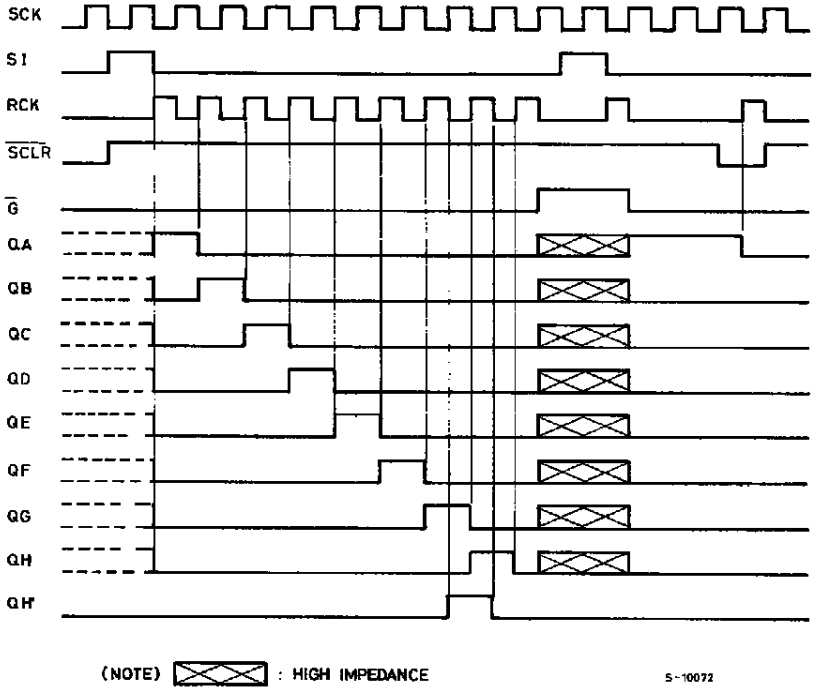
\includegraphics[width=8cm]{./Figures/75hc595_timing.png}
    \caption{Timing diagram of the 74HC595.}
    \label{fig:74hc595_timing}     
\end{figure}

\sourceurl{}{fig:74hc595_timing}{https://cdn-reichelt.de/documents/datenblatt/A240/74HC595\%23STM.pdf}

\noindent As explained in \cref{Ignition Module work} "Controlling the Ignition Circuits" the ignition modules get the information, about what port to fire, over a serial data transmission. The timing diagram in \cref{fig:74hc595_timing} shows how a bit gets shifted though the shift register and outputted by the outputs. This is also the same working principle of the port setting process. However when firing a port, the enable pin(Pin \textit{G} in \cref{fig:74hc595_timing}) of the tri-sate buffer is turned off during the transmission and will only be enabled for $10ms$ after the transmission ended(the ignition time), to fire the set port.\\

\lstinputlisting[frame=l,captionpos=b,firstline=261,lastline=277,caption=Function for transmitting the port to the ignition modules,label=lst:transmit_data]{../../Firmware/ZK_48_Firmware/ZK_48_Firmware.ino}

\noindent The function \textit{transmitData} displayed in \cref{lst:transmit_data} sets the port on all ignition modules. Line 12 till 15 generate a nine impulses long clock signal with a $5 \mu s$ on- and offtime. The reason for nine impulses instead of eight can be explained by viewing \cref{fig:74hc595_timing}. In this timing diagram the shift register clock \textit{SCK} and the register clock \textit{RCK} are 180 Degrees phase shifted, but in \cref{fig:module_circuit} \textit{RCK} and \textit{SCK} are connected together. This means both the shift register clock and register clock receive the clock impulse at the same time. Thus an additional impulse is needed to fully push through the bit, as the register will always be one clock cycle behind. Lines 6 till 10 in \Cref{lst:transmit_data} are setting the data line to high, when the set port is equal to the port. This places the bit in the correct position, to create the desired bit pattern at the shift registers output.

\pagebreak

\subsection{State Machine}
\label{State Machine}

\begin{figure}[!ht]
    \centering
    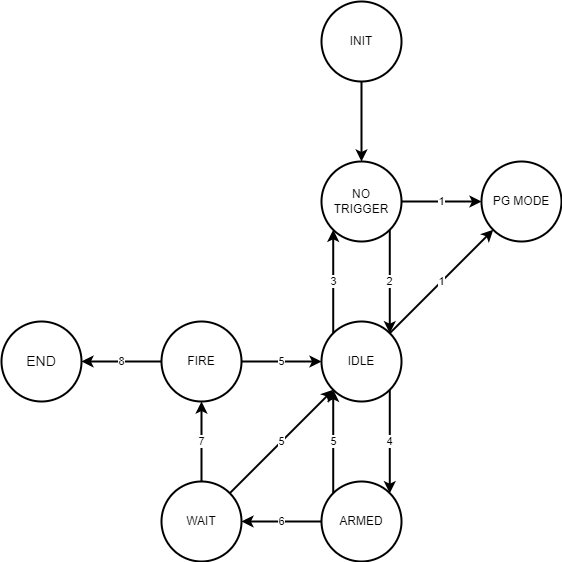
\includegraphics[width=15cm]{./Figures/fsm.png}
    \caption{State diagram of the realised state machine.}
    \label{fig:state_machine}     
\end{figure}

\noindent The firmware starts at INIT and immediately enters NO\_TRIGGER. If no trigger is connected to the controller, the system stays in NO\_TRIGGER until the program mode gets called over USB, or until a trigger is connected. In state IDLE, the systems waits for both arm switches to be armed. If both are armed, the system transitions into ARMED. When in state ARMED, the system waits until it receives a fire signal from the trigger, therefore transitioning to state WAIT. In WAIT, the system stays for $10s$ afterwards it transitions to state FIRE, thus playing through the firing sequence as programmed in EEPROM. When the end is reached, state END is entered and stays there until the device is restarted. If during state FIRE, WAIT or ARMED the controller or the trigger gets unarmed the system returns to state IDLE. This state machine is depicted in \cref{fig:state_machine} together with the transition conditions in \cref{lst:transcond} and the LED and buzzer output for each state in \cref{lst:io_out}.

\pagebreak

\begin{table}[!ht]
\centering
\begin{tabular}{|l|l|l|l|l|} 
\hline
State       &Green&Red&Buzzer&Ontime                           \\ 
\hline\hline
PG\_MODE    &1&1&0& -                               \\ 
\hline
INIT (3x)   &1&1&1& 100ms                           \\
            &0 &0&0& 100ms                           \\ 
\hline
NO\_TRIGGER &1&0&0& 250ms                           \\
            &0&1&0& 250ms                           \\ 
\hline
IDLE        &1&0&0& 100ms                           \\
            &0&0&0& 500ms                           \\ 
\hline
ARMED       &0&1&0& 100ms                           \\
            &0&0&0& 500ms                           \\ 
\hline
WAIT        &0&1&1& 50ms                            \\
            &0&0&0& 50ms                            \\ 
\hline
FIRE        &0&1&1& 10ms (IGNITION\_TIME)            \\
            &1&0&0& \{PROGRAM[PG\_INDEX].DELAY\}ms  \\ 
\hline
END         &0&1&0& -                           \\
\hline
\end{tabular}
\caption{Truth table for the state depended LED and buzzer outputs with timing information.}
\label{lst:io_out}
\end{table}


\begin{table}[!ht]
\centering
\begin{tabular}{|l|l|l|l|l|l|l|l|} 
\hline
Nr & PG & TF & TA & TC & CA & WT & DN  \\ 
\hline \hline
1  & 1  & X  & X  & X  & X  & X  & X   \\ 
\hline
2  & X  & X  & 0  & 1  & 0  & X  & X   \\ 
\hline
3  & X  & X  & X  & 0  & X  & X  & X   \\ 
\hline
4  & X  & X  & 1  & 1  & 1  & X  & X   \\ 
\hline
5  & X  & X  & 0  & X  & X  & X  & X   \\ 
\hline
5  & X  & X  & X  & X  & 0  & X  & X   \\ 
\hline
6  & X  & 1  & 1  & 1  & 1  & 1  & X   \\ 
\hline
7  & X  & X  & 1  & 1  & 1  & 0  & X   \\ 
\hline
8  & X  & X  & X  & X  & X  & X  & 1   \\
\hline
\end{tabular}
\caption{Truth table for the transition condition based on the state variables. ("X" = Don't care)}
\label{lst:transcond}
\end{table}

\subsubsection{State Variables}
\label{State Variables}

\begin{table}[!ht]
\centering
\begin{tabular}{|l|l|l|} 
\hline
State Variable    & SV & Condition                                   \\ 
\hline \hline
Program Mode      & PG & checkPGM()                                  \\ 
\hline
Trigger Fire      & TF & fire\_pulse\_counter >= FIRE\_PULSE\_SETOFF  \\ 
\hline
Done              & DN & pg\_index == pg\_stop                       \\ 
\hline
Wait              & WT & wait\_counter <= FIRE\_DELAY                 \\ 
\hline
Trigger Armed     & TA & digitalRead(TRIGGER\_ARMED)                 \\ 
\hline
Trigger Connected & TC & digitalRead(TRIGGER\_CONNECTED)             \\ 
\hline
Controller Armed  & CA & digitalRead(THIS\_ARMED)                    \\
\hline
\end{tabular}	
\caption{List of all state variables and their conditions}
\label{tab:state_vars_list}
\end{table}


\noindent The state variables listed in \cref{tab:state_vars_list} govern the behaviour of the state machine, as listed in \cref{lst:transcond}. Some state variables are directly read from the IO pins of the Attiny861 and others are the result of internal counter values. In the following paragraphs the state variables will be explained, with the exception of TA, TC and CA as they are generated externally(Please see \cref{fig:controller_circuit} in \cref{Controller}). \\

\pagebreak

\paragraph{PG (Program Mode)}
The program mode state variable is set by a function called \textit{checkPGM()}, which checks if a special keyword is received over USB. In \cref{lst:check_pgm} the code for checking the keyword is depicted.\\

\lstinputlisting[frame=l,captionpos=b,firstline=166,lastline=178,caption=Checking if the keyword for entering the program mode is received.,label=lst:check_pgm]{../../Firmware/ZK_48_Firmware/ZK_48_Firmware.ino}

\noindent The function listed in \cref{lst:check_pgm} reads from the serial(Line 3) stream coming from a external PC and then checks if the string is equal to the keyword(Line 7). The '\#' and ':' are only included due consistency of all instructions. More about the syntax and the instructions in \cref{Instruction Set}.

\paragraph{TF (Trigger Fire)}
To safely detect when the system should fire i.e go into state WAIT, the trigger has to send more than 1000 pulses in under $600ms$ to pin 2 of the Attiny861. Inside the setup function, depicted in \cref{FSetup}, the pin 2 (alias TRIGGER\_FIRE) gets handled by an interrupt, which on signal change, invokes a function called \textit{fire()}. This function is visible in \cref{lst:interrupt}.

\lstinputlisting[frame=l,captionpos=b,firstline=427,lastline=430,caption=Interrupt function for handling the fire signal.,label=lst:interrupt]{../../Firmware/ZK_48_Firmware/ZK_48_Firmware.ino}

\noindent This \textit{fire()} function counts up a variable called \textit{fire\_pulse\_counter}, whereby the value is representing the number of pulses counted. If this counter reaches a value higher than 1000, the TF state variable takes on 1(See \cref{tab:state_vars_list}). Directly after the comparison \textit{fire\_pulse\_counter} must be set to 0, which is shown in \cref{lst:armed} in line 5, which happens $600ms$ after the last comparison.

\paragraph{DN (Done)}
The state variable DN is also the results of the comparison of an up counter and a constant. In \cref{FSetup} \cref{lst:cleardisable} line 3, the program endpoint is read and saved into a variable called \textit{pg\_stop}. This constant stands for the number of steps in the pyrotechnic show. To go through each step of the pyrotechnic show, an up counter is used, incrementing after each firing step is complete. This will be explained in \cref{States} "FIRE". That counter is called \textit{pg\_index} and increments every time state FIRE is called. To generate the state variable DN  \textit{pg\_index} and \textit{pg\_stop} are compared if they are equal DN is 1.

\paragraph{WT (Wait)}
To generate the state variable WT, also a counter is used. This counter, stored in variable \textit{wait\_counter}, counts up every time state WAIT is called. If a threshold called \textit{FIRE\_DELAY} is reached WT takes on logic 1. In \cref{lst:waitcounter} the definition of the \textit{wait\_counter} is visible. Because of the delay of the WAIT state, each call results of a wait time of $100ms$. To generate a $10s$ delay before entering state FIRE, the state WAIT has to be called 100 times, as also explained in the comment in line 1 \cref{lst:waitcounter}.

\lstinputlisting[frame=l,captionpos=b,firstline=75,lastline=76,caption=Definition of \textit{wait\_counter} and the threshold.,label=lst:waitcounter]{../../Firmware/ZK_48_Firmware/ZK_48_Firmware.ino}

\pagebreak

\subsubsection{States}
\label{States}
\paragraph{\textit{PG\_MODE}}
When the program mode or short \textit{PG\_MODE}, is entered the µC sends a special message back to the PC, indicating that \textit{PG\_MODE} was entered successfully. The \textit{PG\_MODE} state consists of a infinite loop calling a function called \textit{programmMode()}, which manages the programming of the pyrotechnic program. This function gets explained in \cref{Program Mode}. In \cref{lst:pgmode} the code of \textit{PG\_MODE} is visible.\\

\lstinputlisting[frame=l,captionpos=b,firstline=327,lastline=332,caption=Code of the \textit{PG\_MODE} state.,label=lst:pgmode]{../../Firmware/ZK_48_Firmware/ZK_48_Firmware.ino}

\paragraph{\textit{INIT}}
\textit{INIT} is entered only once on boot and serves as a visual proof for the user, that the system is booting. Its purpose is to check if all output elements, like the buzzer, red and green LED's are working properly. As visible in \cref{lst:io_out}, all signals will be turned on and off three times, therefore making potential damage to the output elements  visible. In \cref{lst:init} line 1 and 2 the jump conditions are visible.\\

\lstinputlisting[frame=l,captionpos=b,firstline=336,lastline=344,caption=Code of the \textit{INIT} state.,label=lst:init]{../../Firmware/ZK_48_Firmware/ZK_48_Firmware.ino}


\paragraph{\textit{NO\_TRIGGER}}
The state \textit{NO\_TRIGGER} is a major safety features which prevents the system to from directly jumping into the \textit{ARMED} state. When the system is booting and the user forgot to disable the arm switches, the system is prevented to directly jump into the \textit{ARMED} state. This is accomplished by requiring the user to dearm the system before state \textit{IDLE} even can be entered(See \Cref{lst:transcond} Nr. 2 and 3). It not only acts as a safety feature, but also indicates to the user that no trigger is connected, where also the name of the state originated as the safety feature was added later during development. \\

\lstinputlisting[frame=l,captionpos=b,firstline=349,lastline=356,caption=Code of the \textit{NO\_TRIGGER} state.,label=lst:notrigger]{../../Firmware/ZK_48_Firmware/ZK_48_Firmware.ino}

\pagebreak

\paragraph{\textit{IDLE}}
In state \textit{IDLE} the system waits for the user to arm it. Its the return point, if during any further operation the system gets dearmed. Also in \textit{NO\_TRIGGER} and \textit{IDLE} the user can enter the program mode via USB. In \Cref{lst:idle} in line 5 the \textit{wait\_counter} gets reset thus always needing $10s$ to enter state \textit{FIRE} from state \textit{WAIT}.\\

\lstinputlisting[frame=l,captionpos=b,firstline=359,lastline=368,caption=Code of the \textit{IDLE} state.,label=lst:idle]{../../Firmware/ZK_48_Firmware/ZK_48_Firmware.ino}

\paragraph{\textit{ARMED}}
When both arm switches are turned on, the system will transition to state \textit{ARMED}. This state will indicate use the buzzer to notify that the device is armed and ready for operation. If the fire signal is sent and 1000 pulses are counted in under $600ms$ the state \textit{WAIT} is entered (See \Cref{lst:armed}).\\

\lstinputlisting[frame=l,captionpos=b,firstline=372,lastline=380,caption=Code of the \textit{ARMED} state.,label=lst:armed]{../../Firmware/ZK_48_Firmware/ZK_48_Firmware.ino}

\paragraph{\textit{WAIT}}

In \textit{WAIT} the system will wait for $10s$ whilst using the buzzer to warn the user of the upcoming start of the pyrotechnic show, when finally transitioning to \textit{FIRE}. In \Cref{lst:wait} in line 5 the \textit{wait\_counter} gets incremented. 

\lstinputlisting[frame=l,captionpos=b,firstline=385,lastline=394,caption=Code of the \textit{WAIT} state.,label=lst:wait]{../../Firmware/ZK_48_Firmware/ZK_48_Firmware.ino}

\pagebreak

\paragraph{\textit{FIRE}}
When the \textit{wait\_counter} has reached its final value the system transitions into \textit{FIRE} prompting the start of the show. In \Cref{lt:fire} in line 5 the program gets executed by reading in the next port,module and delay to fire and after waiting the read delay firing the next bridge wire detonate in line 10. Afterwards the program counter or \textit{pg\_index} gets incremented to fire the next pyrotechnic effect in the program. This process continues until the program endpoint is reached, as indicated by the DN state variable.\\

\lstinputlisting[frame=l,captionpos=b,firstline=398,lastline=409,caption=Code of the \textit{FIRE} state.,label=lst:fire]{../../Firmware/ZK_48_Firmware/ZK_48_Firmware.ino}

\paragraph{\textit{END}}
The \textit{END} state is the end of the program and will stay stuck in this state until the system gets turned off. It also serves as a safety feature as the system is unable to fire any more, thus making it safe for the user to approach the device after the show has ended.\\

\pagebreak


\subsection{Program Mode}
\label{Program Mode}

The program mode is entered by sending the command "\#PGM:" (See \Cref{State Variables} "PG (Program Mode)") over USB, when the system is in state \textit{IDLE} or \textit{NO\_TRIGGER}. As explained in \Cref{States} "PG\_MODE",  when entering the program mode, the system runs a infinite loop, calling the function \textit{programmMode()} which breaks down a command comming over serial. This is accomplished in three steps: Reading data from Serial, break the command apart and then interpret the broken down command.\\

\lstinputlisting[frame=l,captionpos=b,firstline=183,lastline=186,caption=Reading data from serial.,label=lst:serialread]{../../Firmware/ZK_48_Firmware/ZK_48_Firmware.ino}

\noindent To read data over USB a the function \textit{readString()} is used. This function returns a string containing the content of the serial buffer. Before reading from this buffer, it is necessary to check if data is available, which is done by the function \textit{available()}. On line 4 in \Cref{lst:serialread} a delay with one millisecond is used to slow down the loop as no other delay is present. As TTL serial communication is half duplex, meaning sending and receiving data at the same time is not possible, therefore the delay is preventing a error that sometimes occurs, when reading data and directly afterwards sending data.\\

\lstinputlisting[frame=l,captionpos=b,firstline=188,lastline=197,caption=Break down the command in its parts.,label=lst:serialbreak]{../../Firmware/ZK_48_Firmware/ZK_48_Firmware.ino}


\noindent The next step is to break down the command. For the complete instruction set please read in \Cref{Instruction Set}. A command has always the same structure:\\

\noindent \textbf{\#[CMD-NAME]:[ARG-1]:[ARG-2]:[ARG-3]:[ARG-4]:}\\

\noindent The hashtag at the beginning of the command indicates the start of the command while the colons separate  the arguments. To read the command name and arguments, first the indices of the hashtag and colons are determined by using the \textit{indexOf} method (See \Cref{lst:serialbreak} line 5). This function returns the index of the first char being searched for, starting the search at the entered offset. In this case, the last found index is the offset for the next search(See \Cref{lst:serialbreak} line 7). The found indices are stored in any array for later use. To get the command name as its own string, the \textit{substring} function is utilized, which cuts out a string, given a start index and stop index (See line 10).  \\

\lstinputlisting[frame=l,captionpos=b,firstline=199,lastline=199,caption=Checking if the received command is the \textit{list} command.,label=lst:serialinterpret]{../../Firmware/ZK_48_Firmware/ZK_48_Firmware.ino}

\noindent The command can now be interpreted by having a if-statement, for each command, checking for equality (For an example see \Cref{lst:serialinterpret}). If the received command is equal to one of the commands listed in \Cref{Instruction Set}, its corresponding code is executed.\\

\pagebreak

\subsubsection{\textit{list}}
The \textit{list} command outputs the entire internally stored pyrotechnic show as a list of all steps including the program stop index. This helps the user to check if the pyrotechnic show is programmed correctly or to just see the program itself. The implementation is shown in \Cref{lst:cmdlist}.  
 
\lstinputlisting[frame=l,captionpos=b,firstline=201,lastline=220,caption=Implementation of the \textit{list} command.,label=lst:cmdlist]{../../Firmware/ZK_48_Firmware/ZK_48_Firmware.ino}


\subsubsection{\textit{set}}
For actually programming the pyrotechnic show, the user uses the \textit{set} command. This command takes in four arguments which are all cut out of the buffer (See \Cref{lst:cmdset} line 1-3, 7-9, 11-13, 15-17) by the function \textit{substring} with the indices determined earlier and then stored temporarily in a \textit{section} struct. Finally the struct gets stored in the internal EEPROM (Line 19).\\

\lstinputlisting[frame=l,captionpos=b,firstline=231,lastline=251,caption=Implementation of the \textit{set} command.,label=lst:cmdset]{../../Firmware/ZK_48_Firmware/ZK_48_Firmware.ino}

\pagebreak

\subsubsection{\textit{stop}}
To set the program endpoint alias \textit{pg\_stop}, the \textit{stop} command is used. \textit{stop} has one argument, representing the stop index. This argument converted to an usable integer, by first cutting out the value as a string with the \textit{substring} function (See \Cref{lst:cmdstop} line 1) and then parsing it. The resulting value is then directly written into the internal EEPROM.\\

\lstinputlisting[frame=l,captionpos=b,firstline=224,lastline=227,caption=Implementation of the \textit{stop} command.,label=lst:cmdstop]{../../Firmware/ZK_48_Firmware/ZK_48_Firmware.ino}


\subsubsection{Instruction Set}
\label{Instruction Set}

\begin{table}[ht!]
\centering
\begin{tabular}{|l|l|} 
\hline
Command                                & Description                                              \\ 
\hline \hline
\#pgm:                                 & Enters the program mode \\ 
\hline
\#list:                                & Lists the stored pyrotechnic program\\ 
\hline
\#set:[INDEX]:[MODULE]:[PORT]:[DELAY]: & Sets a point in the pyrotechnic program\\ 
\hline
\#stop:[STOP\_INDEX]:                  & Sets the end of the pyrotechnic program\\
\hline
\end{tabular}
\caption{List of all commands}
\label{tab:instruction_set}
\end{table}

\pagebreak